% !TeX spellcheck = en_US
\addscenariosection{1}{Clash Scenario}{Dragon Valley}{\images/slayer.png}

\begin{multicols*}{2}

\textbf{Author:} LAAMAKALA

\textbf{Source:} \href{https://discord.com/channels/740870068178649108/1239631918643941509}{Archon Studios Discord}

\textit{The valley calls to those who seek adventure and riches beyond imagination. Its heart is guarded by Dragons older than time, its edges lined with settlements of those who dare to claim a foothold in this perilous land. But there is no safety here—only the promise of power for those who fight, and the certainty of death for those who falter.}

\subsection*{\MakeUppercase{Scenario Length}}
This Scenario is played over 13 Rounds (or a shorter version over 8 Rounds).

\subsection*{\MakeUppercase{Player Setup}}
\textbf{Player Count:} 2 -- 4

\textbf{Starting Resources:} 15 \svg{gold}, 4 \svg{building_materials}, 2 \svg{valuables}

\textbf{Starting Income:} 10 \svg{gold}, 0 \svg{building_materials}, 0 \svg{valuables}

\textbf{Starting Units:}
\begin{itemize}
  \item A Few \svgunit{bronze} Units of the player's choice
  \item A Pack of \svgunit{bronze} Units of the player's choice
\end{itemize}

\textbf{Town Buildings:} 
\begin{itemize}
  \item \svgunit{bronze} Dwelling
  \item Each player may build the \textit{Mage Guild} or a \textit{Faction-specific} building with a discount of 10 \svg{gold} (trading post conversion chart may be used for the discount)
\end{itemize}

\subsection*{\MakeUppercase{Map Setup}}
Take the following Map Tiles and arrange them as shown in the Scenario map layout ($P$ stands for the number of players):

\begin{itemize}
  \item P × Starting (I) Map Tile
  \item 3P × Far (II-III) Map Tiles - one per player must include a Settlement, and one per player must include a Trading Post
  \item 2P × Near (IV-V) Map Tile
\end{itemize}

\textbf{Additionally, for 2--3 players:}
\begin{itemize}
  \item 1 × Center (VI-VII) Map Tile with a Dragon Utopia
\end{itemize}

\textbf{For 4 players:}
\begin{itemize}
  \item 2 × Center (VI-VII) Map Tiles with a Dragon Utopia
  \item P × Center (VI-VII) Map Tiles containing Settlements and Grails
\end{itemize}

\subsection*{\MakeUppercase{Victory Conditions}}
The game ends at the end of the Round when any of these conditions are met:

\begin{itemize}
 \item One player has defeated all other players' Main Heroes once - \textit{That player wins the game immediately.}
 \item One player conquers both Dragon Utopias - \textit{That player wins the game immediately.}
 \item At the end of Round 13 (or Round 8 for the shorter game).
\end{itemize}

\subsection*{\MakeUppercase{Victory Points}}
If no player has achieved an immediate victory, the player with the most Victory Points (VP) wins:

\begin{itemize}
 \item 5 VP for conquering a Dragon Utopia
 \item 4 VP for controlling 5 Mines or Settlements on Near and Center Tiles - \textit{once per game}
 \item 4 VP for defeating an enemy's Main Hero - \textit{once per defeated Faction}
 \item 2 VP for defeating an enemy's Secondary Hero - \textit{once per defeated Faction}
 \item 2 VP for each enemy Main Town captured - \textit{once per captured Faction}
 \item 1 VP for every controlled Mine or Settlement
 \item 1 VP for every Level of Experience of your Main Hero
\end{itemize}

\subsection*{\MakeUppercase{Timed Events}}

\begin{itemize}
  \item Start of \textbf{\nth{1} and \nth{9} Rounds:} All Heroes gain +1 Movement.
  \item Start of \textbf{\nth{4} and \nth{8} Rounds:} Remove black Cubes from all locations that give resources, morale or Cards.
  \item End of \textbf{\nth{10} Round:} Player(s) with lowest XP roll 2 Resource dice.
\end{itemize}

\subsection*{\MakeUppercase{Additional Rules}}
\begin{itemize}
  \item Remove ``Earthquake'', ``Remove Obstacles'', ``View Earth'', and ``Visions'' from the Spell Deck.
  \item Remove ``Unexpected Reinforcements'' from the Astrologers Proclaim Deck.
  \item Make one Deck of minor, one of major and one of relic artifacts.
  \item Make one Deck of basic spells and one of expert spells.
  \item On Starting and Far Tiles players can only get basic spells and minor artifacts.
  \item Players may not use Diplomacy to skip lvl VII Combat.
  \item If your Hero is lvl VII, treat lvl VI neutrals as lvl VII and gain 10 \svg{gold}
  \item Sanctuary effect: +1 Morale and draw 1 Card. Visitable once per Faction.
  \item Obelisk effect: Roll one Resource die and draw one Card. \textit{May be visited once per Faction.}
  \item When fighting a neutral Combat, a player may add +1 difficulty for an extra 5 \svg{gold} + Search (2) the Artifact or the Spell Deck
  \item Level VII settlements are treated as two settlements for rewards AND roll one Resource or Treasure (reroll any XP) die.
  \item If a player defeats neutral Units on a Grail hex, he immediately gets: 10 \svg{gold}, 4 \svg{building_materials} and 2 \svg{valuables}. (alternative: Throw 2 treasure (reroll any XP ) and 2 Resource dice)  \textit{Can be conquered only once.}
  \item Dragon Utopia: Reshuffle the \svg{gold} and \svg{azure} Decks, then draw \svg{azure} until you get 3 Dragons and choose 2 AND draw from \svg{gold} until you get one Dragon. 
  \item When a player conquers Dragon Utopia, he may recruit one of the neutral Dragons killed for half the \svg{gold} (rounded down) + \svg{valuables} OR gain 15 \svg{gold} AND Search (3) any artifact Deck. \textit{Can be conquered only once.}
\end{itemize}

When a Dragon Utopia is conquered, roll an attack die:
\begin{itemize}
  \item -1: The defeated Dragons’ spirits curse the land! All players lose 1 MP for the next Round.
  \item  0: Dragons revenge: All players must sacrifice one Unit before the end of Round, that Unit's health is reduced to 0. 
  \item +1: Scattered Treasure: All players may immediately lose 1 MP to Search (2) the artifact Deck.
\end{itemize}

\subsection*{\MakeUppercase{Suggested houserules}}
\begin{itemize}
  \item Trading Posts - Trade resources and remove Cards, OR buy war machines.
  \item Unlimited combat Rounds against neutrals + harder Level. +gain combat lvl × \svg{gold}.
  \item \href{https://boardgamegeek.com/thread/3445901/custom-hex-combat-board}{Medium Hex combat board}.
  \item \href{https://boardgamegeek.com/thread/3449937/houserule-for-stacking-more-than-pack}{Medium Hex combat board} - Start with several Few \svg{bronze} Units.
\end{itemize}

\vspace*{\fill}

\end{multicols*}

\begin{tikzpicture}[overlay]
  \centering
  % 2-player
  \node at (4.5, -5) {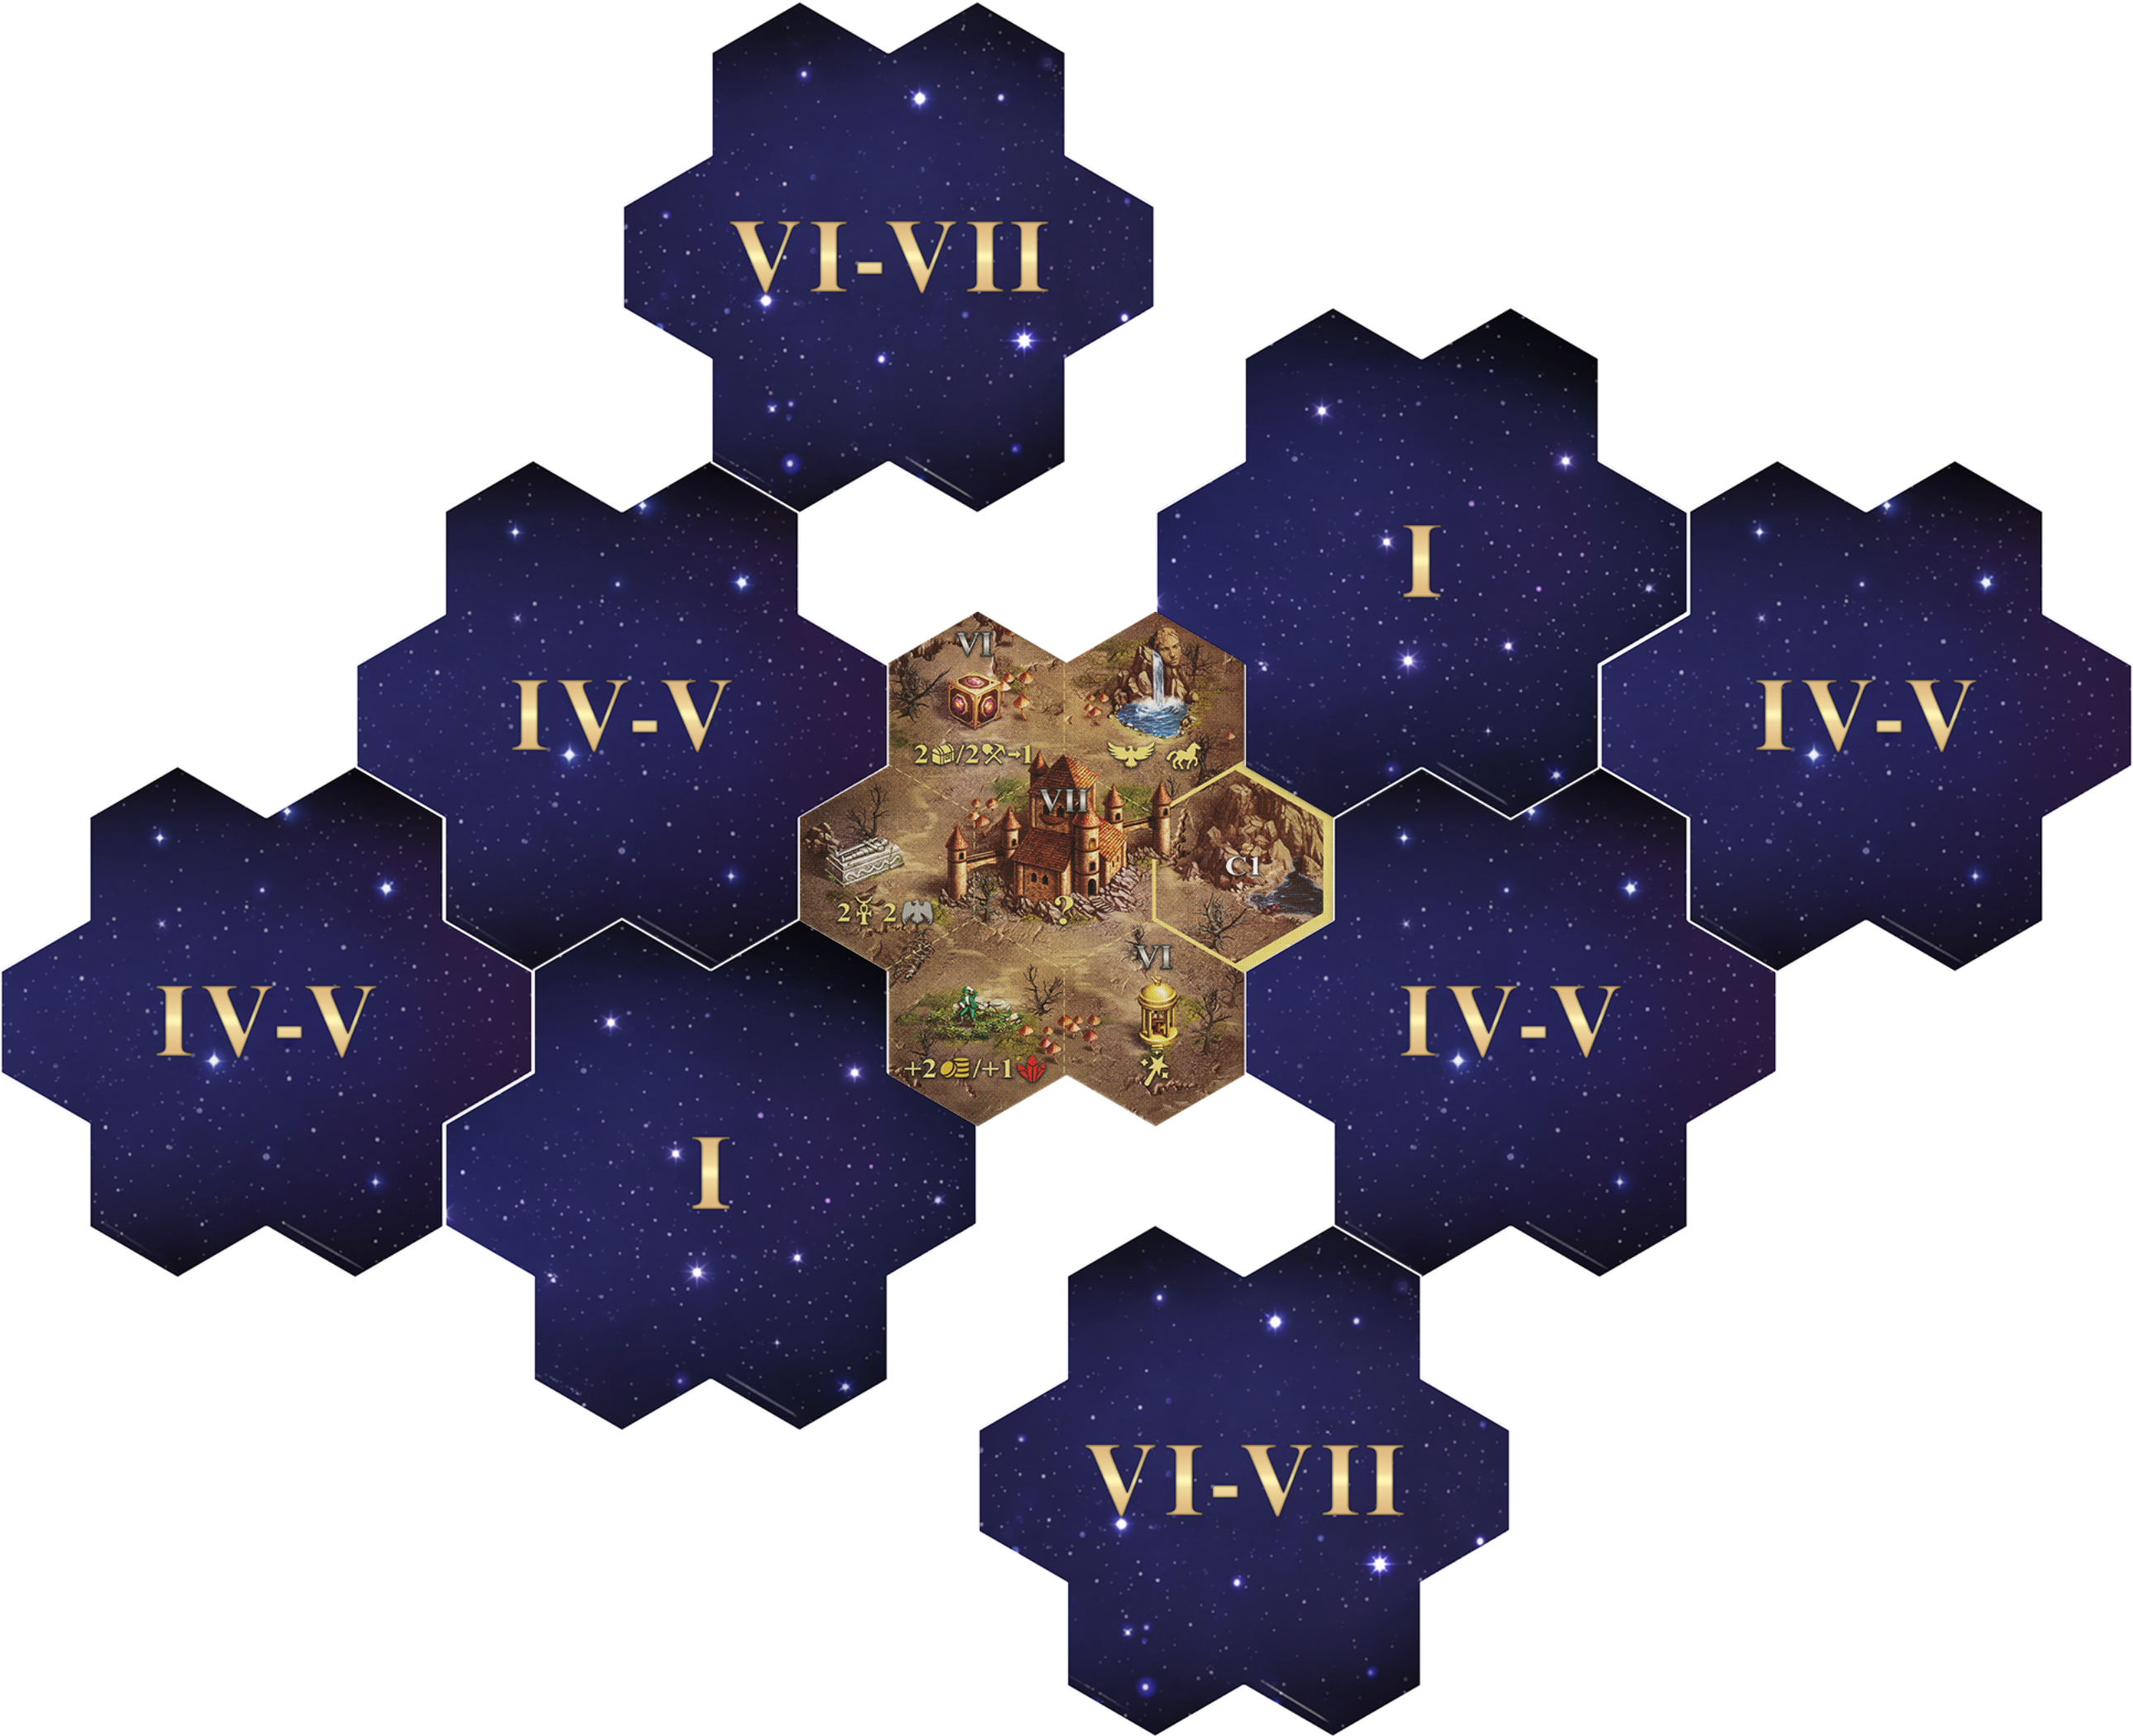
\includegraphics[scale=0.165]{\maps/dragon-valley-2p.png}};
  \node at (4.5, -10) {\footnotesize{\textbf{\MakeUppercase{2-PLAYER SCENARIO}}}};
  % 3-player
  \node at (12.1, -5) {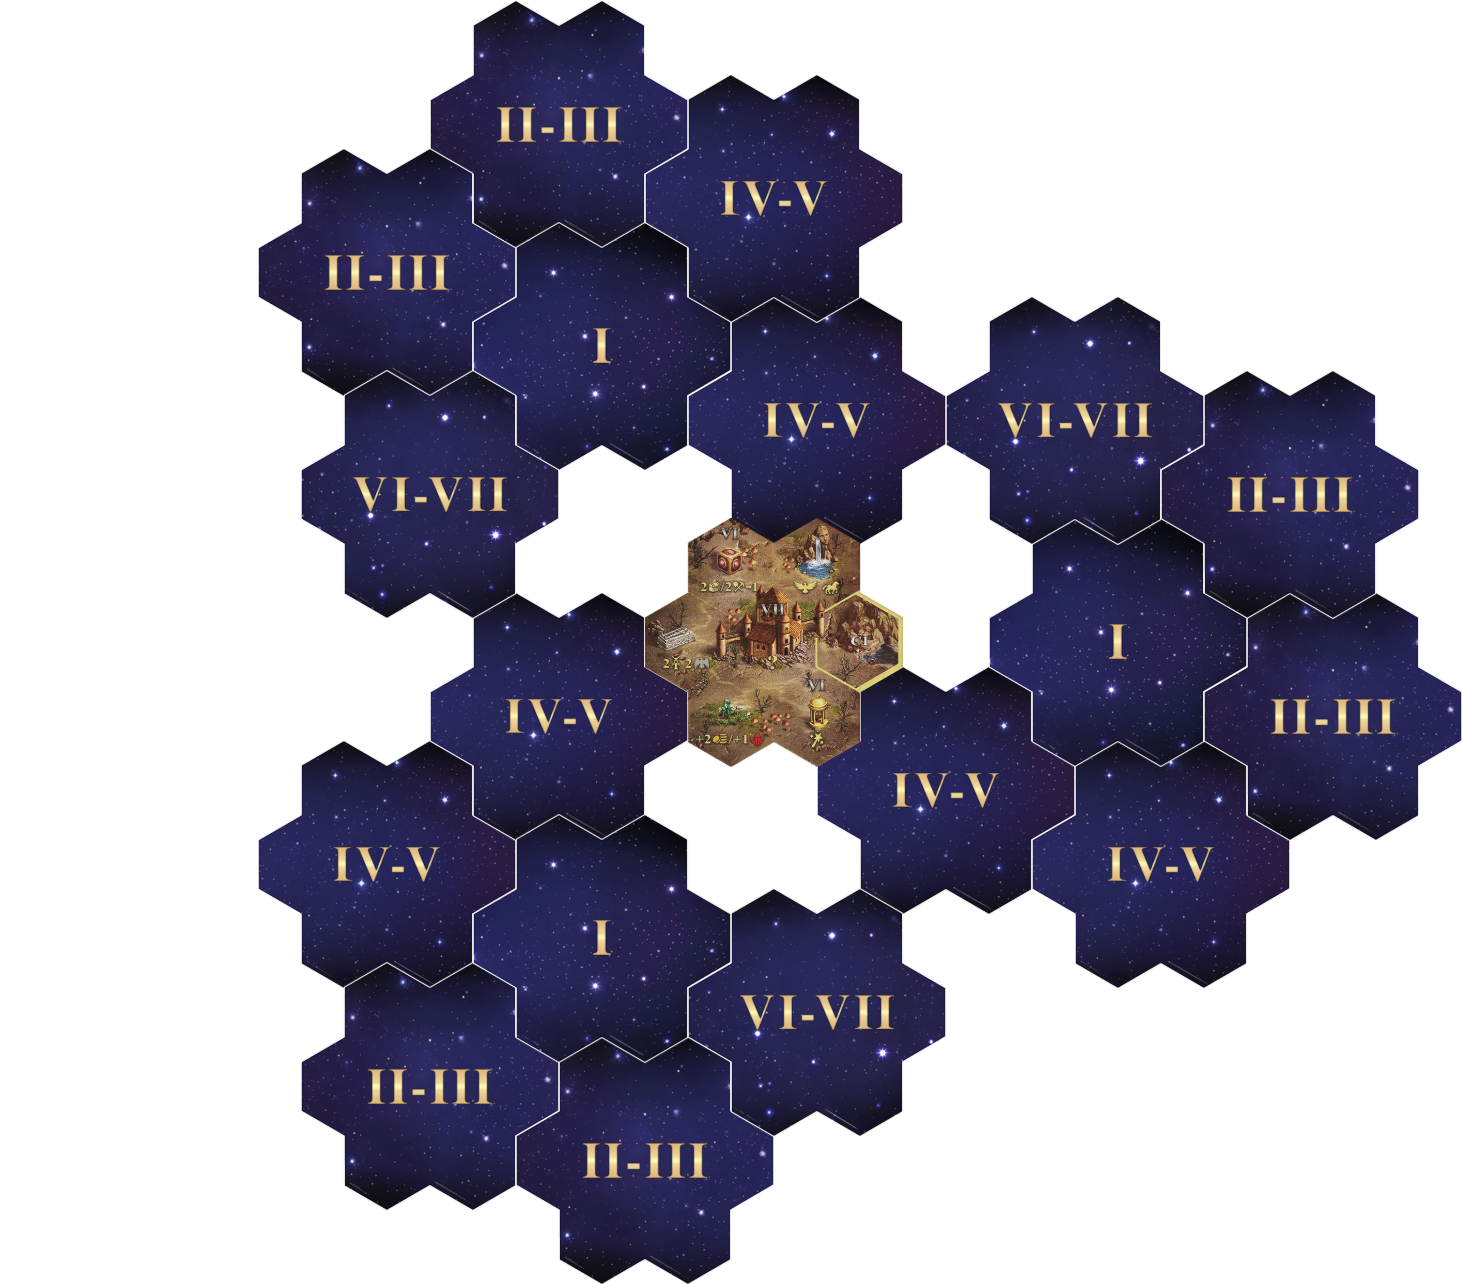
\includegraphics[scale=0.165]{\maps/dragon-valley-3p.png}};
  \node at (12.1, -10) {\footnotesize{\textbf{\MakeUppercase{3-PLAYER SHORT SCENARIO}}}};
  % 4-player
  \node at (4.5, -15) {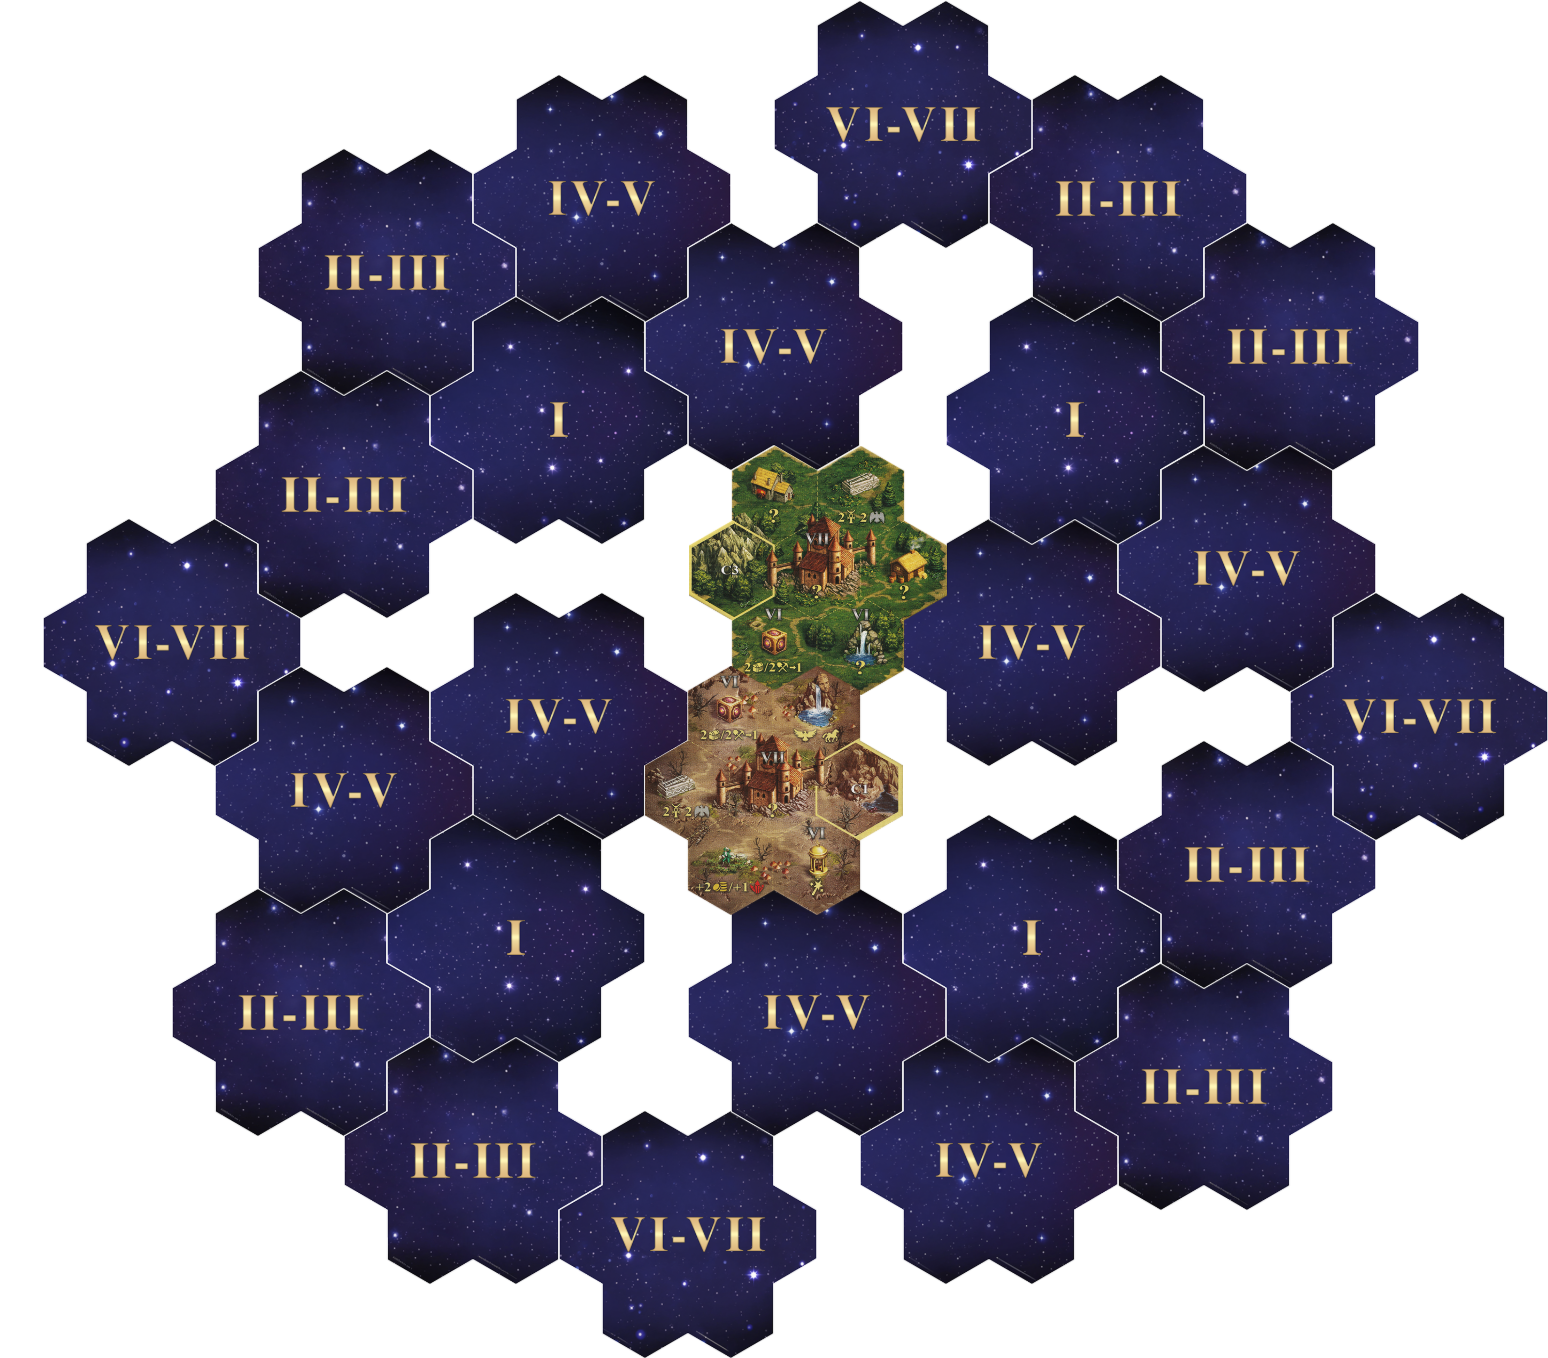
\includegraphics[scale=0.165]{\maps/dragon-valley-4p.png}};
  \node at (4.5, -20) {\footnotesize{\textbf{\MakeUppercase{4-PLAYER SCENARIO}}}};
  % 4-player short
  \node at (12.1, -15) {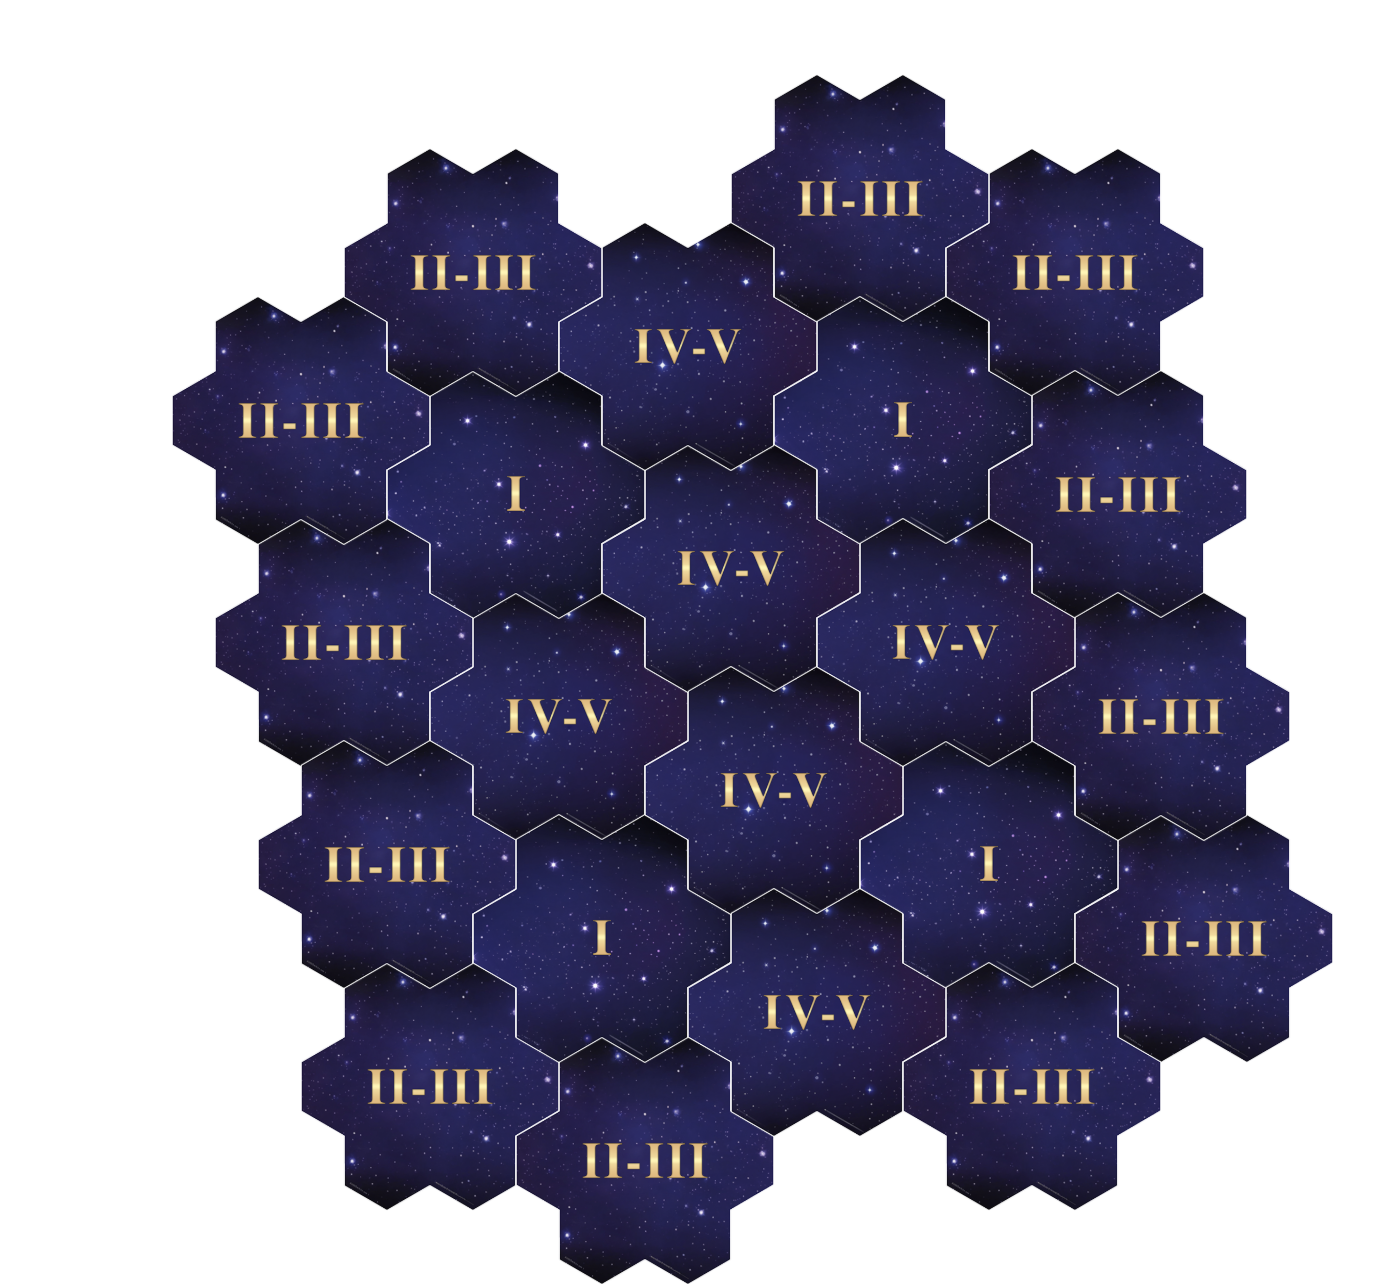
\includegraphics[scale=0.165]{\maps/dragon-valley-4p-short.png}};
  \node at (12.1, -20) {\footnotesize{\textbf{\MakeUppercase{4-PLAYER SHORT SCENARIO}}}};
\end{tikzpicture}
